
%\subsection{Cultural Significance of Facades and Ornament}
%\label{subsec: FacadeandOrnament}

%%==========================
%%Delve deeper into how facades reflect cultural values, societal norms, and historical contexts. Explore how different societies and civilizations have expressed their identity through architectural ornamentation and symbolism.
%%==========================
We have established a foundation for the notion that contemporary architecture is gravitating towards a renaissance of complexity.
This resurgence is catalyzed by the utilization of technology and sophisticated software analyses, enabling the creation of innovative ornamentation that seamlessly integrates functionality with cultural heritage.
This evolution paves the way for the elaboration of intricate patterns that serve as a powerful medium to express the distinct identity of the local environment, thereby rejuvenating the urban landscape.

Transitioning into the focal point of this research, we delve into the trajectory of architectural complexity within the specific realm of facades.

Facades, a paramount architectural element, have held an enduring significance for centuries due to their role as the initial point of contact with a building, acting as a boundary between the interior and the exterior, working as an interface between the living spaces and the external climate, influencing comfort and energy efficiency\cite{Kamal2020} thereby acting as the primary medium through which the structure interacts with its surroundings (Figure\ref{fig:FacadeBaroqueVsContemporary}).

%% Figure of baroque facade vs contemporary facade
     \begin{figure}[htb]
          \centering
          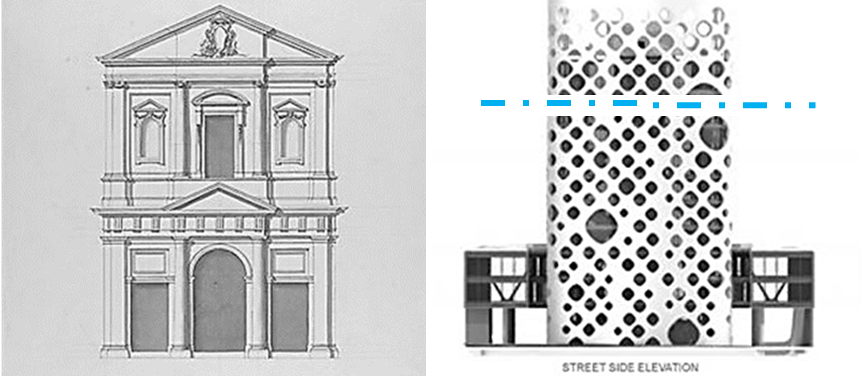
\includegraphics[width= \linewidth]{Images/BaroqueVsContemporaryfacade}
          \caption{Evolution of facade design.
          Baroque Facade 1639 by Bernini (left) vs Contemporary facade, building O-14 by Reiser + Umemoto, 21st Century (right) (\textit{Images edited from source)}}
          \label{fig:FacadeBaroqueVsContemporary}
        \end{figure}

However, much like the broader scope of architecture, the role of ornamentation and facades has also undergone evolution and transformation throughout history.
To elucidate how various societies and civilizations have conveyed their identity through architectural ornamentation and symbolism, we embark on an exploration of the interpretations given to facades by some of the most influential architects and artists of their respective eras.

%%Facade according to vitruvius

Vitruvius, a celebrated Roman architect and military engineer, in 1st century BCE, author of ``De Architecura'', a series of ten books considered as the first treatise in architecture theory\cite{Kruft1994}.
Within this work, Vitruvius advocates for three essential attributes that a building should embody: ``firmitas'' (structural soundness), ``utilitas'' (functionality), and ``venustas'' (beauty or aesthetics)\cite{Ostwald2023}.

Vitruvius places emphasis primarily on Reason, and secondarily on proportions.
It's worth highlighting that the cultural atmosphere in ancient Rome during the late first century B.C favoured the understanding of the world as a well-structured and ordered whole\cite{Lefas2000}.

Facades partake of this reasoning and in accordance to Vitruvius should not only be visually appealing but should also reflect the underlying structural integrity of the building and fulfill its intended purpose effectively(Figure\ref{fig:Vitruvianarchitecture}).
In terms of ornamentation, Vitruvius seeks to approach this subjective realm, dominated by taste, with objectivity.
He rationalizes that a pleasing appearance emerges from the harmony and balance among the components that constitute a composition\cite{Lefas2000}.

%% Figure of vitruvian Architecture
    \begin{figure}[htb]
        \centering
        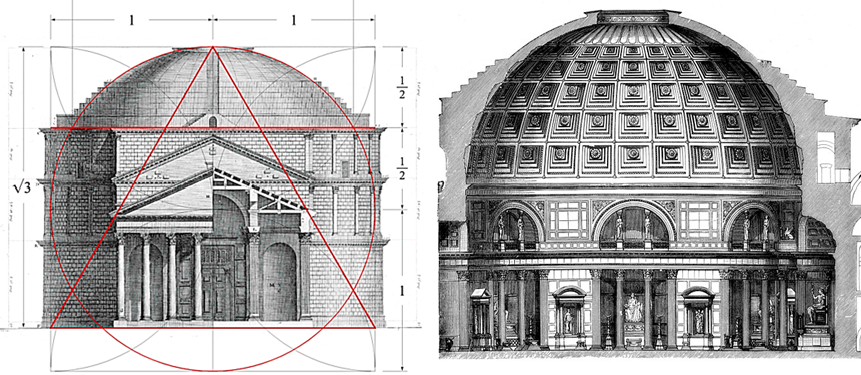
\includegraphics[width= \linewidth]{Images/VitruvianArchitecture}
        \caption{Facade and ornament according to Vitruvius, with emphasis in order symmetry and harmony. Pantheon's facade (left) and cross section(right) symmetry analysis (\textit{Images edited from source)}}
        \label{fig:Vitruvianarchitecture}
    \end{figure}

Additionaly, Vitruvius determines that the deciding factor for those components would follow the principle of ``Decor'',  the  fifth  principle on his system of values that elevates simple  building  practice  into  architecture, defined as the property that  deals  with  the  «appropriate»  articulation and construction of the work on principles respecting religion, nature and social conventions\cite{Lefas2000}.

In essence, according to Vitruvius, facades and their ornamentation stem from a sense of order and rationality.
They are achieved through a harmonious equilibrium of well-considered elements that adhere to established principles, while taking into account both tradition and nature.
This approach aims to achieve beauty while also effectively fulfilling the intended purpose of the facade.

Vitruvius's contributions would have a lasting impact on the field of construction spanning centuries.
However, his work remained largely dormant for a considerable period until its revival during the Renaissance.
This resurgence led to the rekindling of Classical architecture in the years that followed\cite{Wikipedia2023}.

%%facade according to bernini and borromini
Moving beyond the Renaissance era and into the Baroque style, a significant shift in the perception of facades and ornamentation occurs.
Francesco Borromini, a prominent Italian architect of the Baroque period, emerges as a key figure in this context.

In his exploration of facades, Borromini emphasized the dynamic relationship between a building's interior and its facade, as a form of movement of matter beyond the body, precisely because the generation of form is internal to the object itself\cite{Benjamin2006}, therefore the facade should serve as a visual representation of the internal spaces and functions of the building.

Borromini's approach to facades went beyond mere decorative elements.
He saw the facade as an opportunity to express the inner workings and spatial organization of the building.
This concept is reflected in his designs, where facades often featured intricate geometric patterns, curved forms, and sculptural elements that hinted at the internal arrangements of rooms and structures(Figure\ref{fig:BorrominiArchitecture}).

%% Figure of Baroque facade Borromini
     \begin{figure}[htb]
          \centering
          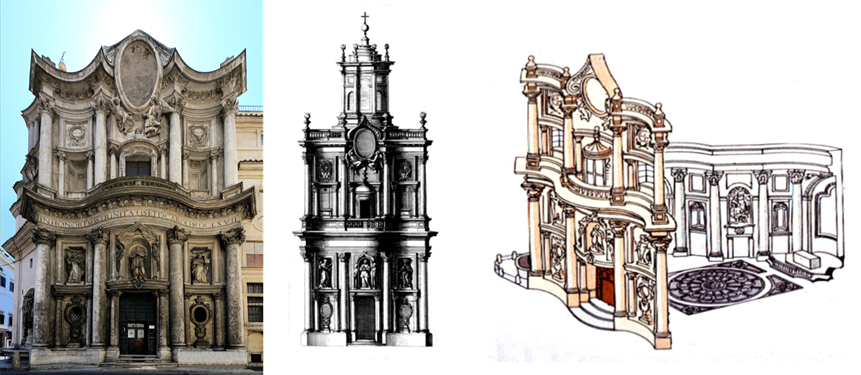
\includegraphics[width= \linewidth]{Images/BaroquefacadeBorromini}
          \caption{Borromini's Interpretation of Facade and Ornament: Elaborate geometric patterns, curved forms, and sculptural elements reflecting internal spatial arrangements. Analysis of San Carlo alle Quattro Fontane Church Facade (left) and Cross Section (right) from its construction in the 1630s, Rome. (\textit{Images edited from source)}}
          \label{fig:BorrominiArchitecture}
        \end{figure}

``Exteriors which expressively display interiorities;
interiors which fold from within and, [\ldots] which appear to invite an exterior reading while presenting an interiorized text''\cite{Biglieri2004}.
In essence, Borromini's perspective on facades went beyond surface aesthetics;
he considered them as integral components of the architectural composition that could convey deeper meanings about the building's design and purpose.

%% context on bypassing neo classic and art deco

By delving into the historical evolution of facades and ornamentation, it's essential to acknowledge certain periods that contributed to our understanding without undergoing radical shifts.
Neo-Classical and Art Deco styles, for instance, added to the discourse around facades and ornament, albeit without fundamentally altering prevailing paradigms .

The Neoclassical style of mid 18th century was a reflection of Facade and Ornament derived from Vitruvian Principles and Palladian Architecture, while the ArtDeco style prevalent in Europe and America during in the 1920s to early 1930s will come to rethink Facade and Ornament through the Prisms of Luxury and Technological Progress.

The goal was to evoke a sense of modernity while also paying homage to the past, resulting in a fusion of historical references and futuristic aspirations (Figure\ref{fig:NeoclassicArtDeco}).

%% Figure of Neo classic style ornament and Art Deco style  facade
     \begin{figure}[htb]
          \centering
          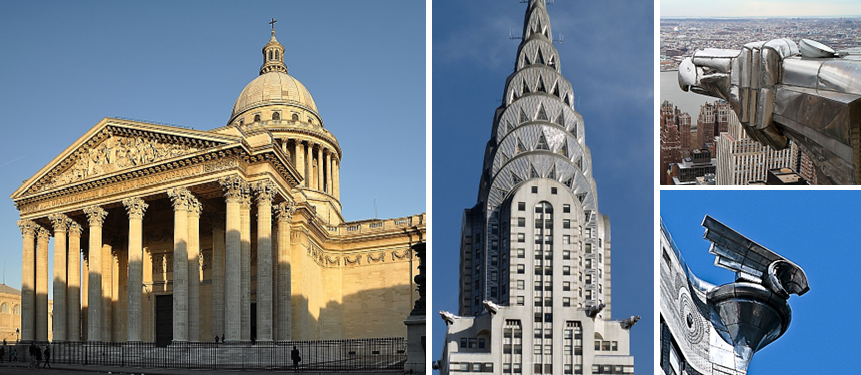
\includegraphics[width= \linewidth]{Images/NeoclassicArtDeco}
          \caption{(Left) Neoclassical Approach in the Mid-18th Century: illustrated by the Paris Pantheon, constructed between 1758 and 1790. (Right) Art Deco Approach in the 1920s to Early 1930s: Exemplified by the Chrysler Building and its Ornamental Details, completed in 1930. (\textit{Images edited from source)}}
          \label{fig:NeoclassicArtDeco}
        \end{figure}

With this broader context established, the analysis will now shift its focus to the Modernist movement's transformative impact on architectural philosophy.

%%facade according to le corbusier

Transitioning from the Baroque style, where facades became expressions of internal dynamics, and acknowledging the enriched insights from the Neoclassical and ArtDeco Style,  the historical evolution of facades and ornamentation takes us into the Modernist style of the 20th century—a pivotal juncture that marked one of the most significant shifts in architectural theory.

 Within this era, a radicalized interpretation of ``Form follows function'' emerged, embodying a profound departure from the conventional understanding of facades and ornamentation, partly due to a prevailing stance against ornamentation, often dismissed on moralistic grounds.

Adolf Loos' 1908 article ``Ornament and Crime'' exemplified this sentiment by advocating functional design and condemning conventional ornamentation as unnecessary\cite{Saglam2014}.

Le Corbusier, one of the most prominent figures of this epoch, and renowned for his influential work ``Towards a New Architecture'' first published in 1923, and considered by some to be the most important architectural work published in the 20th century, epitomized the spirit of the era with his distinct views on facades and ornamentation\cite{Studio2a2023}.

Embracing a minimalist and utilitarian approach, Le Corbusier believed that a facade should mirror a building's internal functions, designed in alignment with its purpose and occupants' needs.

Rooted in a human-centric design philosophy, his mantras ``Constructing the architecture of men'' and ``Men are the ones who truly matter'' underscored his commitment to prioritizing people's well-being in his designs\cite{Virseda2021}.

His manifesto ``The Five Points of a New Architecture'' further solidified his design principles.
The notion of ``Free design of the facade'' attained by separating the exterior of the building from its structural function is presented as the means through which the facade liberates itself from conventional structural\cite{Corbusier1986}.

This allowed for the incorporation of large expanses of windows to provide ample natural light and ventilation, fostering a seamless connection between the interior and exterior realms.

Even during this era when ornamentation was viewed unfavorably, Le Corbusier believes in a form of functional ornamentation, as Venturi\cite{Venturi1972} would later accurately point out, Modern architecture uses expressive ornament and shuns explicit symbolic  ornament.

He would ingeniously devise methods to infuse his creations with a distinct form of ornamentation, albeit one rooted in materials' textures, structural elements, and inventive ways of articulating functionality\cite{Saglam2014} that emerged from the building's design.

For example, he used sunshades, brise-soleil, and other shading devices as a way to address climate and control light without compromising the building's aesthetic integrity.

In essence, Le Corbusier's viewpoint on facades and ornamentation epitomized clarity, rationality, and harmonious integration.
His architecture rejected superfluous adornment, and celebrated both technological advancements and structural innovation while maintaining a genuine focus on the well-being and experiences of the occupants (Figure\ref{fig:Modernistfacade}).

%% Figure of Modernist facade and ornament by Le corbusier
     \begin{figure}[htb]
          \centering
          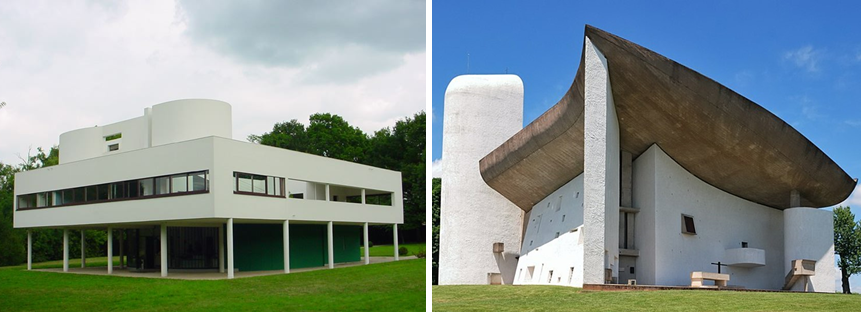
\includegraphics[width= \linewidth]{Images/ModernistFacade}
          \caption{Evolution of Functionalism: Le Corbusier's Journey towards Modernist Facade and Ornamentation. (Left) Villa Savoye, 1928-1931. (Right) Chapelle Notre-Dame-du-Haut de Ronchamp, 1955 (\textit{Images edited from source)}}
          \label{fig:Modernistfacade}
        \end{figure}


%%facade according to Venturi

However, despite the innovative ideals of the Modernist movement,  it became apparent that its utopian vision didn't always materialize as intended.
While the pursuit of functionalism and simplicity was meant to create efficient and logical designs, the outcomes were not always aligned with the intended human experiences.

The Modernist approach often led to the unintentional creation of spaces that felt monotonous and detached from their cultural contexts.
The emphasis on minimalism and the rejection of ornamentation sometimes resulted in environments lacking a sense of identity and character.

The architectural pursuit of universality and timelessness would instead produce sterile, glass-cube structures\cite{Schudel2018} disregarding the importance of cultural heritage and local context, and inadvertently raise the question: Is the reinvention of form, that rejected explicit symbolism and frivolous applique ornament, inspired by the modernist ideals,  yielding a Heroic and original outcome, or is it, instead, a dry expressionism, empty and boring that has distorted the whole building into one big ornament\cite{Venturi1971}.

This scrutiny of the Modernist movement's inability to adequately encompass human experiences and cultural significance, which sparked controversy during the 1960s, brings us to the influential ideas of architect and theorist Robert Venturi.

Venturi's book ``Complexity and Contradiction in Architecture'', published in 1966, marked a turning point in architectural discourse and challenged the prevailing modernist ideals.

Robert Venturi, an iconoclastic architect often hailed as the pioneer of postmodernism\cite{Schudel2018} stood firmly against the oversimplification of architecture, championing the incorporation of contradiction and complexity to yield authentic and vital creations.

The modernist ideals, heavily favoring automobile-centric urban planning, influenced the formation of cities that catered to cars rather than people.
In their thought-provoking book from 1972, "Learning From Las Vegas," Venturi et al.\cite{Venturi1972} put forth a compelling argument, exemplified by the stark contrast seen in places like Las Vegas, they assert that if you were to strip away the dazzling signs, what remains is not a thriving urban environment but a barren desert, illustrating the detachment of architecture relegated to a mere functional necessity camouflaged behind attention-grabbing signs.

Venturi et al.\cite{Venturi1972} will further explain that the oversimplification of architecture, combined with the emergence of sprawling spaces, high speeds, and intricate functions where symbols hold more significance than actual forms, has transformed architecture into symbols occupying space, rather than forming it.

This shift implies that the architectural structure itself carries minimal meaning, with the focus primarily directed towards the signs that communicate with it.

The building stands isolated from the street, often separated by vast parking lots, while the front-facing sign juts out perpendicular to the highway, detached from the building.
At the rear, the structure becomes a utilitarian afterthought, reduced to a budgetary obligation\cite{Venturi1972}.

In this scenario, the absence of signs leaves behind a vacuous atmosphere, characterized by scattered buildings that lack enclosure and cohesion.
The architecture loses its essence, mirroring a cultural void much like a desert devoid of life and enrichment.

The impact of these dynamics is not confined to the past;
instead, they continue to reverberate through the present state of our cities.
Many urban landscapes today still adhere to the principles that emerged from the modernist era.
The prioritization of cars and the resulting sprawling infrastructure persist in shaping cityscapes that often prioritize functionality over human experience.

In response to the challenges posed by the Modernist movement and its unintended consequences, Venturi would reshape the course of architectural discourse.
Notably, he will famously invert the famous dictum of Mies van der Rohe ‘Less is more’ into ‘Less is a bore'\cite{Lutolli2020}, encapsulating his bold departure from the prevailing architectural norms.

In his book ``Complexity and Contradiction in Architecture''\cite{Venturi1977}, Venturi emphasized that architecture should be responsive to the cultural context and the people who inhabit it.

His viewpoint marked a departure from the rigid modernist principles who shunned symbolism of form as an expression or reinforcement of content that dictated that architectural form was to be determined solely by program and structure, with an  occasional  assist from  intuition\cite{Venturi1972}, instead he proposed a reevaluation of the role of ornament and complexity in architectural design (Figure\ref{fig:postmodernfacade}).

%% Figure of Postmodernism facade and ornament
     \begin{figure}[htb]
          \centering
          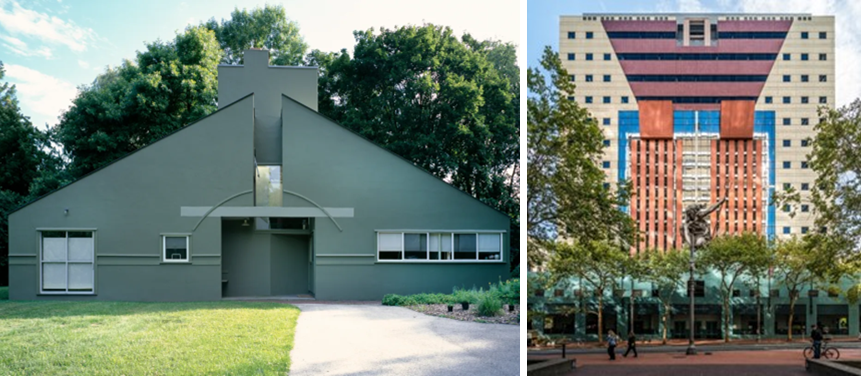
\includegraphics[width= \linewidth]{Images/PostmodernismVenturi}
          \caption{Postmodernism and the advent of complexity and contradiction (Left) Vanna Venturi House, designed by Robert Venturi and Denise Scott Brown in 1964. (Right) Portland Municipal Services Building, designed by Michael Graves, in 1982 (\textit{Images edited from source)}}
          \label{fig:postmodernfacade}
        \end{figure}

On this context, Venturi believed that a facade could communicate various meanings, evoke emotions, and respond to its cultural and contextual surroundings.
Venturi emphasized the richness of symbolism within architecture, asserting that symbols were fundamental in the architectural language, advocating for the integration of elements from historical precedents and the existing urban fabric, treating them as source materials that could be intelligently referenced or replicated to inform the design process\cite{Venturi1971}.

Importantly, Venturi's approach did not solely prioritize outward appearance;
it was deeply intertwined with the functional aspects of a building's interior, aligning with his belief that architecture should serve both utilitarian purposes and evoke meaningful experiences.

Regarding ornament, he argued that ornamentation was not inherently negative but should be used judiciously and meaningfully.
Venturi coined phrase ``Less is a bore'', suggests his approach towards ornament in what he would later refer to as "the decorated shed"\cite{Venturi1972} ing that architecture doesn't have to be stripped of ornamentation to be considered valid.
He encouraged architects to embrace complexity, contradiction, and the richness of historical references in their designs.

In other words, Robert Venturi's views on facades and ornament emphasized the importance of embracing diversity, historical references, and meaning in architectural design, he wants modern architects to realize only one thing— perfection in the architectural world can and should include imperfection, in all its forms\cite{Lutolli2020}.
=============================
%% reorganize the venturi text and seprate it from the critic of modernism. Add a las vegas analyses pic or something related to the soulless architecture. revision the interpretation of facades and ornament with citations before progressing into the contemporary

%%i need to add a paralel that our cities were generated under the modernist ideals and preference of the car which lead to the reference to Las vegas and how if you remove the signs, there is no place only a desert due to the disengage of architecture now reduce to a cheap necessity hidden behind the sign. Also add a picture of the postmodern style with a reference towards facade and ornament made clear in similar fashion as the conclusions of style written before that ussually start with in essence.

%I want to make a reflection at this point, the modernist movement utopia failed and resulted in the creation of monotonous places desensatized from its culture.
%the functionalism was misinterpreted as plainliness and resulted in dehumanized elements.
%the focus on light and glass facades ignored contextual relationship where the climate unapologetically would turn this glass boxes into ovens pradoxical ignoring the maxim of human centric design.
%architecture would follow a pattern regardless of its roots and connection to its local making them virtually indistinguishable from one another in striking contrast to the richful global diversity of the past.
%the absence of ornament was misinterpreted as the lack of effort reducing architecture to mere construction.

   %%%==========================References


    Venturi wants modern architects to realize only one thing— perfection in the architectural world can and should include imperfection, in all its forms\cite{Lutolli2020}.


    In Complexity and Contradiction in Architecture, Robert Venturi tries to give counter-arguments to the modernist approach. He advocates embracing ‘contradiction and complexity’ to create valid, vital works.\cite{Lutolli2020}

    It is noteworthy that he doesn’t oppose aesthetic simplicity. What he rejects is the ‘oversimplification’ of architecture, indicated when he inverted the famous Mies van der Rohe statement ‘Less is more’ into ‘Less is a bore’.\cite{Lutolli2020}

    Modern architects, who shunned symbolism of form  as  an expression or reinforcement of content: meaning was  to  be  communicated,  not  through  allusion  to  previously  known forms, but through the inherent, physiognomic characteristics of form.
    The creation of architectural form was to be a logical process, free  from images  of past experiences, determined solely by program and structure, with an  occasional  assist,  as  Alan Colquhoun has  suggested, from  intuition.
    But some recent critics  have  questioned  the possible level of content to  be derived  from  abstract forms.
    Others have  demonstrated that the functionalists,  despite  their protestations, derived  a  formal vocabulary of their own, mainly from current art movements and the industrial vernacular;
    and  latter-day  followers  such  as  the  Archigram  group  have turned,  while  similarly  protesting,  to Pop  Art and  the space  industry.\cite{Venturi1972}

    Because the spatial relationships are made by symbols more than by forms, architecture in this landscape becomes symbol in space rather than form in space.
    Architecture defines very little: The big sign and the little building is the rule of Route 66.
    The sign is more important than the architecture.
    This is reflected in the proprietor's budget the sign at the front is a vulgar extravaganza, the building at the back, a modest necessity.
    The architecture is what is cheap.\cite{Venturi1972}

    The little low buildings, gray-brown like the desert, separate and recede from the street that is now the highway, their false fronts disengaged and turned perpendicular to the highway as big, high signs.
    If you take the signs away, there is no place.
    The desert town is intensified communication along the highway.\cite{Venturi1972}

    Ugly and ordinary as symbol and style
    Heroic and Original, or ugly and ordinary

    Robert Venturi, an iconoclastic architect often considered the father of postmodernism who rejected sterile, glass-cube structures in favor of an inclusive, eclectic style that embraced community values and a touch of vulgarity\cite{Schudel2018}

    He turned Mies van der Rohe’s famous dictum about simplicity in design — “Less is more” — upside down, cheekily declaring, “Less is a bore.”\cite{Schudel2018}

    Mr. Venturi’s declaration of architectural values, “Complexity and Contradiction,” was a manifesto that took aim at the prevailing modernist notion that architecture should aspire to a cold, glassy perfection with cold, glassy buildings.
    He argued instead that architecture should reflect changing times and social needs.
    The world of design, he said, had too long been in the grip of the dogma that architects were godlike creators who could impose their vision on the landscape.\cite{Schudel2018}

     Las Vegas wasn’t just a neon-lit den of vulgarity, they concluded.
     It was a prime example of a city built to accommodate the automobile.
     As a result, signs were often more important than the buildings they loomed over.\cite{Schudel2018}

    “In the landscape of the automobile, the architecture becomes insignificant, a pimple on the landscape of parking lots,” Mr. Venturi told the Times in 1971.\cite{Schudel2018}

    He never lost his disdain for what he considered the soulless architecture of his modernist predecessors, who often designed glass-box buildings with walls of windows, “but you would never have a wall with a window in it.”\cite{Schudel2018}

    Instead, Mr. Venturi wrote in “Complexity and Contradiction in Architecture,” he drew inspiration from the “everyday landscape, vulgar and disdained,” which was “valid and vital for our architecture as a whole.”\cite{Schudel2018}

    some architects wanted to move away from minimalist glass and steel and return to the ornamentation of the past. Postmodernists such as Michael Graves, James Stirling, Robert Venturi, and Denise Scott Brown responded to the work of their predecessors with bold buildings that showcased color and references to classical design. [...] Discover five of the most influential buildings of the postmodern movement and see how their eclectic and innovative designs pushed the boundaries of architecture in the 20th century\cite{Stamp2016}.


    %
    According to Krier the mature city achieves balance with nature and with the people that it serves in its scale, size and integration of residential, commercial and civic functions.
    Krier argues that the reconstruction of a city is a moral imperative, a global project that it is at once cultural social economic and ecological. Time of video 1:06:29\cite{Economakis2023}